\documentclass[border=2pt]{standalone}

\usepackage{tikz}

\usetikzlibrary{positioning}

\begin{document}
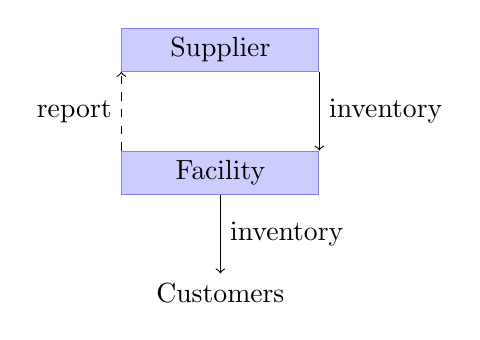
\begin{tikzpicture}
  [place/.style={rectangle,draw=blue!50,fill=blue!20,
                 minimum width=25mm,align=center}]
  \node[place] (supplier)                      {Supplier};
  \node[place] (facility)  [below=of supplier] {Facility};
  \node        (customers) [below=of facility] {Customers};

  \draw [->,dashed] (facility.north west) -- node[auto] {report}
                    (supplier.south west);
  \draw [->] (supplier.south east) -- node[auto] {inventory}
             (facility.north east);
  \draw [->] (facility) -- node[auto] {inventory}
             (customers);
\end{tikzpicture}
\end{document}
